\chapter{Architettura}

In questo capitolo verranno descritte le scelte architetturali e implementative che stanno alla base del contributo di questa tesi al progetto IoE. 

Lo scenario legato alla mobilità elettrica veicolare è caratterizzato dalla presenza di diversi domini applicativi, piattaforme e parti interessate i quali necessitano di comunicare in modo unificato e trasparente. A tal fine è stato utilizzato il progetto Smart-M3 (\cite{tullio2011}), cuore della nostra architettura. Appoggiandosi sulle tecnologie tipiche del \emph{Semantic Web}, Smart-M3 assicura l'interoperabilità tra gli attori in gioco. 

In particolare vedremo come possono coesistere elementi reali ed elementi simulati e come il passaggio dall'uno all'altro sia assolutamente trasparente a tutti i componenti del sistema grazie all'uso di tecnologie ontology-based.

\section{Smart-M3}\label{sec:smart-m3}

Prima di parlare dei componenti strettamente legati a questo progetto è doveroso fare un introduzione alla tecnologia che fa da collante tra di essi, ovvero Smart-M3. Capire come funziona Smart-M3 e quali sono i suoi principi è fondamentale per comprendere a fondo il seguito di questo documento.

M3 è un architettura middleware che realizza l'interoperabilità delle informazioni in maniera cross-domain, multi-vendor, multi-device, multi-piattaforma (\cite{smart2013}). Smart-M3 è la sua prima implementazione Open Source, proposta da SOFIA, un Progetto Europeo (2009-11) appartenente al framework ARTEMIS. 
La piattaforma implementa il disaccoppiamento tra produttori e consumatori di informazione. In questa architettura tutti gli attori (sensori, dispositivi, servizi, attuatori ecc..) cooperano attraverso un database RDF che è lo standard deciso dal World Wide Web Consortium per la descrizione di informazioni e concetti. L'interoperabilità è resa possibile da un modello di dati condiviso che si basa su tecnologie tipiche del Semantic Web.

Il Semantic Web è un framework sviluppato dal World Wide Web Consortium per consentire la condivisione e il riutilizzo dei dati attraverso  applicazioni, aziende e comunità eterogenee.

La figura \ref{fig:smart-m3} mostra il funzionamento dell'architettura M3. Il ``legacy gate'' è un interfaccia con il mondo esterno e possono coesisterne molteplici istanze in un architettura M3.

\begin{figure}[H]
	\centering
	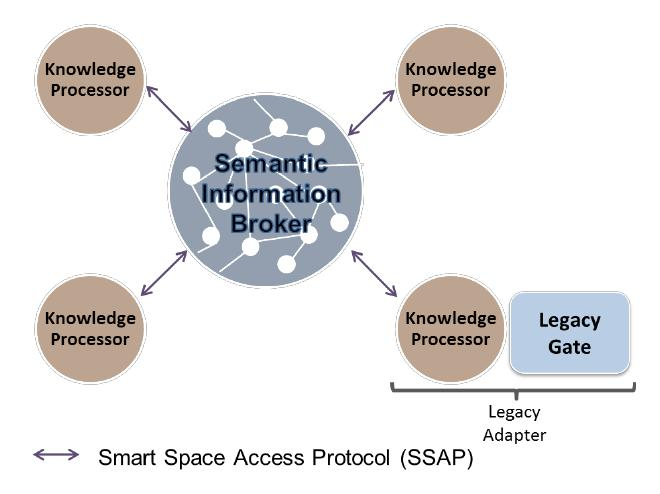
\includegraphics[width=0.5\textwidth]{assets/smart-m3.jpg}
	\caption{Architettura Smart-M3}
	\label{fig:smart-m3}
\end{figure}

\subsection{Semantic Information Broker}\label{subsec:sib}

Il \emph{Semantic Information Broker} (SIB) è l'entità responsabile della conservazione e della gestione delle informazioni condivise nell'architettura M3. Gli agenti Software che si scambiano le informazioni vengono chiamati \emph{Knowledge Processors} (KP). L'accesso alla SIB da parte dei KP avviene attraverso lo \emph{Smart Space Access Protocol}  (SSAP) basato su messaggi XML scambiati attraverso socket TCP/IP. Vengono fornite API che implementano il protocollo SSAP in diversi linguaggi.

Il SIB è un architettura a 5 livelli (\cite{smart2010}) come mostrato in figura \ref{fig:sib-architecture}:

\begin{enumerate}
	\item \textbf{Transport}: Gestisce una o più comunicazioni di rete a livello di trasporto, permettendo al SIB di comunicare con diverse reti e architetture. Il livello di trasporto è collegato a quello sottostante tramite il DBus, rendendo possibile l'aggiunta e la rimozione di connettori a runtime.
	\item \label{enum:handling}\textbf{Operation Handling}: Gestisce le diverse operazioni del protocollo SSAP ognuna delle quali viene eseguita in un thread dedicato. Malgrado l'uso intensivo di thread possa degradare le performance,  è stata ritenuta determinante la chiarezza di codice che ne consegue.
	\item \label{enum:graph}\textbf{Graph Operations}: Gestisce le operazioni di inserimento, rimozione e query dal database RDF come richiesto dal livello \ref{enum:handling}. Viene eseguito all'interno di un singolo thread che schedula ed esegue le richieste provenienti dai thread che gestiscono le operazioni SSAP la cui comunicazione avviene tramite code asincrone.
	\item \textbf{Triple Operations}: Gestisce le operazioni SPARQL, WQL e le query basate su pattern-matching di triple RDF. Attualmente è implementato tramite Piglet, un database RDF che si appoggia ad SQL lite per la persistenza delle informazioni. Lo strato può essere tranquillamente cambiato a patto che si scriva il codice necessario ad interfacciare le operazioni a livello di grafo (\ref{enum:graph}) con l'interfaccia fornita dal nuovo store RDF.
	\item \textbf{Persistent storage}: Assicura la persistenza dei dati.
\end{enumerate}

\subsection{I Knowledge Processor}\label{subsec:kp}

I Knowledge Processor (KP) sono le parti attive dell'architettura Smart-M3. Un KP interagisce con il SIB non direttamente tramite il protocollo SSAP ma tramite le Knowledge Processor Interface (KPI) ovvero le librerie che lo implementano. Queste possono trovarsi a qualunque livello di astrazione ed essere scritte in qualunque linguaggio. Le funzioni messe a disposizione dal KPI in genere sono speculari alle operazioni del protocollo SSAP.

I KP sono le entità che forniscono, modificano e richiedono le informazioni le informazioni contenute nello smart-space. L'architettura dei KP è mostrata in figura \ref{fig:kp-architecture}.

\begin{figure}[H]
        \centering
        \begin{subfigure}[H]{0.5\textwidth}
                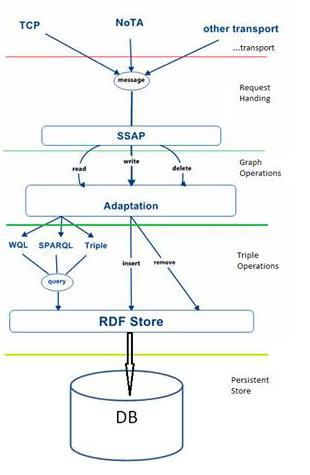
\includegraphics[width=\textwidth]{assets/sib-architecture-2.jpg}
                \caption{Architettura del SIB}
                \label{fig:sib-architecture}
        \end{subfigure}%
        \begin{subfigure}[H]{0.42\textwidth}
                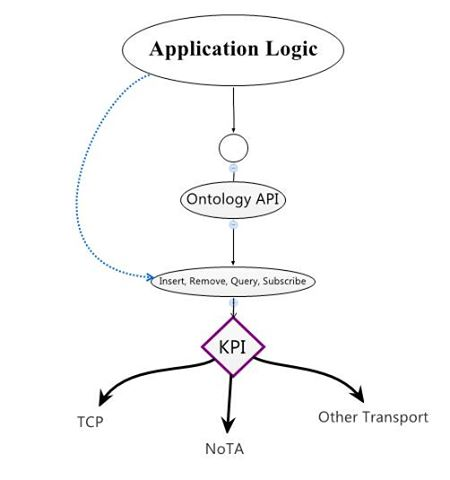
\includegraphics[width=\textwidth]{assets/kp-architecture.jpg}
                \caption{Architettura dei KP}
                \label{fig:kp-architecture}
        \end{subfigure}
        \caption{Architetture SIB e KP}
\end{figure}

\subsection{Le triple RDF}

Nell'architettura Smart-M3 le informazioni sono rappresentate in formato RDF (Resource Description Framework). In RDF le informazioni sono rappresentate in forma di triplette \emph{soggetto, predicato, oggetto}. Le triple vengono memorizzate nel SIB e formano un grafo etichettato diretto che non necessariamente è un grafo connesso.

\subsection{Ontologie}

Mentre RDF fornisce il modello di dati standard per la rappresentazione delle informazioni, l'uso di un linguaggio ontologico è indispensabile per assegnare una semantica all'informazione. Linguaggi ontologici come RDFS e OWL forniscono un vocabolario comune. L'uso di una ontologia comune consente a tutti gli attori (uomini e macchine) di capire reciprocamente la semantica delle informazioni e di cooperare in simbiosi attraverso il SIB. Smart-M3 è agnostico rispetto all'ontologia e quindi consente agli sviluppatori di scegliere il modo migliore di modellare le informazioni per soddisfare le esigenze funzionali del dominio applicativo indirizzato.

\subsection{Sottoscrizioni}

Un aspetto fondamentale di questa tecnologia è il meccanismo delle sottoscrizioni grazie al quale è possibile ricevere notifiche al variare di set di triple. Le sottoscrizioni sono determinanti nella nostra architettura perché, come vedremo più avanti (Sez. \ref{sec:protocol}), sono alla base dei protocolli di scambio dati tra i componenti del sistema.

\subsection{SPARQL}

\emph{SPARQL}  (pronuncia sparkle, acronimo ricorsivo di SPARQL Protocol and RDF Query Language) è il linguaggio standard de facto per interrogare dataset RDF. Come si può dedurre dal nome stesso, SPARQL non è semplicemente un linguaggio di interrogazione di dati RDF ma definisce anche il protocollo applicativo utilizzato per comunicare con le sorgenti RDF (si tratta di un binding su HTTP).

Così come SQL riflette nella rappresentazione della query il modello relazionale sottostante, allo stesso modo SPARQL basa la rappresentazione della query sul concetto di tripla e di grafo. Il meccanismo alla base della rappresentazione di una query e della ricerca della sua risposta è il graph matching. La query rappresenta un pattern di un grafo (RDF) e la risposta alla query sono tutte le triple (sotto-grafo) che \emph{fanno match} con il pattern.

\subsection{Il protocollo SSAP}

L'SSAP (\emph{Smart Space Access Protocol}) è il protocollo con cui si comunica con il SIB. Essendo un protocollo session-based, i KP che vogliono comunicare con lo smart-space dovranno prima aderirvi con un operazione di Join prevista dall'SSAP. Il KP fornisce le sue credenziali nel messaggio di Join, il SIB esamina le credenziali e decide se accettare il KP o meno. Dopo l'operazione di Join, il KP può eseguire le altre operazioni. 
L'SSAP è il punto di integrazione principale dell'architettura Smart-M3. Le implementazioni di SIB e KP devono implementare tutte le operazioni del protocollo SSAP per garantire l'interoperabilità.

Le operazioni supportate dal protocollo SSAP sono:

\begin{itemize}
	\item \textbf{JOIN}: Associa il KP allo smart-space solo se le credenziali vengono ritenute valide. Determina l'inizio della sessione.
	\item \textbf{LEAVE}: Determina il termine dell'associazione con lo smart-space e quindi la fine della sessione. Da questo momento in poi non potranno essere eseguite altre operazione di associazione allo smart-space.
	\item \textbf{INSERT}: Operazione atomica di inserzione di un Grafo, formato da triple RDF, nel SIB.
	\item \textbf{REMOVE}: Operazione atomica di rimozione di un Grafo, formato da triple RDF, nel SIB.
	\item \textbf{UPDATE}: Operazione atomica di aggiornamento di un Grafo, formato da triple RDF, nel SIB. In realtà si tratta di una combinazione di DELETE e INSERT eseguita in modo atomico con precedenza dell'operazione di DELETE.
	\item \textbf{QUERY}: Richiesta di informazioni contenute nel SIB attraverso una delle modalità supportate.
	\item \textbf{SUBSCRIBE}: Sottoscrizione a un set di triple contenute nel SIB. Il KP riceve una notifica quando avviene un cambiamento su una di queste triple.
	\item \textbf{UNSUBSCRIBE}: Cancella una sottoscrizione.
\end{itemize}

%\begin{figure}
%	\centering
%	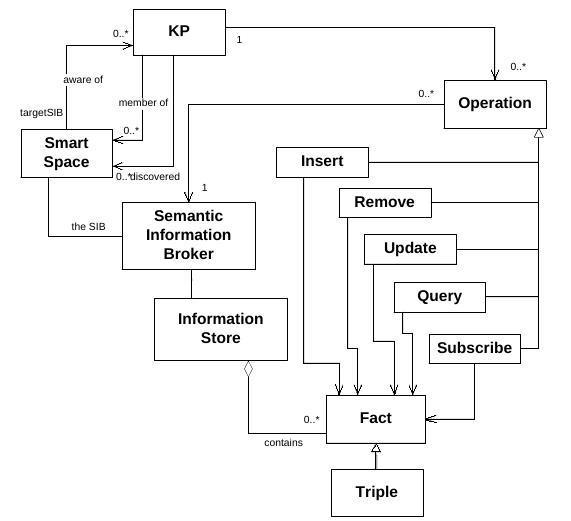
\includegraphics[width=0.5\textwidth]{assets/smart-m3-domain.jpg}
%	\caption{Smart-M3 modello di dominio}
%	\label{fig:smart-m3-domain}
%\end{figure}

\section{Il Modello Ontologico}

In questa sezione cercherò di illustrare come sono stati modellati i dati attraverso una ontologia. Ho ereditato dalla progetto di Tesi di \emph{Federico Montori} (\cite{montori2012}). Io ho contribuito espandendolo per adattarlo ai nuovi requisiti funzionali sorti durante lo sviluppo del progetto. Verranno quindi mostrati gli aspetti dell'ontologia necessari per comprendere il resto della trattazione e verranno approfondite le modifiche da me apportate.

\subsection{Introduzione}

L'ontologia è definibile come una rappresentazione formale ed esplicita di una concettualizzazione condivisa di un dominio di interesse.

L'ontologia presenta le seguenti proprietà:

\begin{itemize}
	\item \textbf{Rappresentazione Formale}: come tale usa un linguaggio logico processabile da elaboratori.
	\item \textbf{Esplicita}: cioè non ambigua e tale da chiarire ogni assunzione fatta.
	\item \textbf{Concettuale}: è una concettualizzazione cioè una vista astratta e semplificata del dominio di interesse.
	\item \textbf{Condivisa}: determinata dal consenso di una pluralità il più ampia possibile di soggetti.
\end{itemize}

Lo scopo delle ontologie è quindi descrivere delle basi di conoscenze, effettuare delle deduzioni su di esse e integrarle tra le varie applicazioni. Per descrivere le ontologie viene utilizzato il linguaggio OWL (\emph{Ontology Web Language}), estensione di RDF. È un linguaggio di markup per rappresentare esplicitamente significato e semantica di termini con vocabolari e relazioni tra gli stessi.

I linguaggi della famiglia OWL sono in grado di creare \emph{classi}, \emph{proprietà}, \emph{istanze} e le relative \emph{operazioni}.


\subsection{Classi di IoE}

Una classe è una collezione di oggetti che corrisponde alla descrizione logica di un concetto. Da una classe si possono creare un numero arbitrario di istanze mentre ad un istanza possono corrispondere una, nessuna o molteplici classi.

Una classe può essere sottoclasse di un'altra classe, ereditando le caratteristiche della super-classe. Tutte le classi sono sottoclasse di \code{owl:Thing}, rappresentazione concettuale di ``cosa''.

Nel modello di dati utilizzato in questo progetto si è cercato di tenere disaccoppiato il concetto di dato dalle altre entità fisiche. Ne consegue che tutte le entità fisiche sono sottoclassi dirette di \code{owl:Thing}, mentre le classi destinate a rappresentare i dati sono sottoclassi di \code{ioe:Data} che a sua volta è sottoclasse di \code{owl:Thing}.

Nel resto di questo documento userò il prefisso \code{ioe:} come abbreviazione di \emph{http://www.m3.com/2012/05/m3/ioe-ontology.owl\#} il namespace scelto per l'ontologia. In generale userò questo prefisso per distinguere le classi dell'ontologia dalle classi Java che come vedremo nella sezione \ref{subsec:ioe-lib} hanno lo stesso nome essendo mapping diretto di quest'ultime.

\subsection{Sottoclassi di owl:Thing}\label{subsec:thing}

Come già accennato tutte le entità fisiche del nostro modello ontologico sono sottoclasse diretta di owl:Thing. Quella mostrata di seguito è una lista delle Classi usate in questo progetto omettendo quelle attualmente irrilevanti o inutilizzate.

\begin{description}
	\item \code{ioe:Person}: rappresenta il concetto di persona. Ad ogni persona possono essere associati diversi veicoli (\code{ioe:Vehicle}), diverse richieste di ricarica (\code{ioe:Reservation}) nonché la storia delle ricariche effettuate (\code{ioe:Recharge}). Il concetto di persona viene usato ai fini dell'autenticazione e in un futuro potrà essere determinante ai fini della fatturazione che il provider energetico eseguirà a fronte delle ricariche.
	\item \code{ioe:Vehicle}: rappresenta il concetto di Veicolo Elettrico. I veicoli NON elettrici sono infatti irrilevanti al fine di questa trattazione. Ad ogni veicolo sono ovviamente associati i dati della batteria (\code{ioe:BatteryData}) che verranno trattati nella sezione relativa alle sottoclassi di \code{ioe:Data} (\ref{subsec:ioe-data});
	\item \code{ioe:Zone}: rappresenta l'area di copertura del \emph{City Service}. È definita da un rettangolo individuato dagli angoli nord-ovest e sud-est. 
	\item \code{ioe:GridConnectionPoint}: il \emph{Grid Connection Pointer} (\code{ioe:GCP}) è la stazione di ricarica. Contiene almeno un EVSE, rappresentazione della colonnina dove avviene la ricarica effettiva. Il rapporto tra un GCP e gli EVSE è lo stesso che intercorre tra una stazione di rifornimento e le pompe di benzina. 
	\item \code{ioe:EVSE}: Il \emph{Electrical Vehicle Supply Equipment} è il punto in cui il veicolo si connette alla rete elettrica. Una volta connesso può sia ricaricare la sua batteria che cedere energia alla Grid. Un EVSE ha diversi connettori (\code{ioe:Connector}) per adattarsi ai vari tipi di presa in dotazione ai veicoli elettrici. Inoltre ogni EVSE dispone di una lista di prenotazioni associate.
	\item \code{ioe:ChargeProfile}: è l'insieme dei parametri che caratterizzano il profilo energetico di un EVSE in un determinato istante. I parametri attualmente sono: potenza, orario di validità del profilo stesso e prezzo per unità di energia (in genere 1 kWh). Può essere attivo un solo \code{ioe:ChargeProfile} alla volta, variabile opzionalmente in base a fasce orarie analogamente a quanto avviene per l'energia elettrica casalinga.
	\item \code{ioe:Connector}: è il connettore di ricarica ovvero il tramite tra l'EVSE e l'EV. Ogni EVSE può avere diversi connettori per la massima compatibilità col maggior numero di veicoli possibile. Malgrado negli USA si stia cercando di introdurre uno standard, esistono ormai diversi tipi di connettori. 
	\item \code{ioe:ChargeRequest}: Richiesta di ricarica. Viene istanziata quando un utente deve creare una prenotazione. Al suo interno sono contenuti tutti i parametri necessari a descriverla. Fa parte del protocollo di richiesta di prenotazione discusso nella Sez. \ref{sec:protocol}. Un approfondimento sulla sua struttura è trattato nella Sez. \ref{subsubsec:chargerequest}.
	\item \code{ioe:ChargeResponse}: è la risposta fornita dal servizio cittadino a seguito della richiesta di prenotazione. Al suo interno contiene un riferimento alla richiesta (\code{ioe:ChargeRequest}) da cui è stata generata e una lista di opzioni di ricarica conformi alla richiesta dell'utente (\code{ioe:ChargeOption}).
	\item \code{ioe:ChargeOption}: Fa parte della risposta(\code{ioe:ChargeResponse}) che il servizio cittadino da all'utente in seguito a una richiesta di prenotazione (\code{ioe:ChargeRequest}). Contiene i parametri di ricarica quali EVSE, orario e prezzo. 
	\item \code{ioe:Currency}: rappresenta la divisa monetaria relativa a un prezzo. Alcune sue istanze sono state inserite direttamente nell'ontologia (\code{ioe:Euro}, \code{ioe:Dollar} ecc..);
	\item \code{ioe:Reservation}: viene creata un istanza di questa classe se il protocollo di richiesta di prenotazione va a buon fine. Indica che l'EVSE a cui è associata è impegnato per un certo lasso di tempo. 
	\item \code{ioe:ReservationList}: lista di prenotazioni associate ad un EVSE. Ogni EVSE può avere un unica lista di prenotazioni associata.
	\item \code{ioe:ReservationRetire}: classe che denota la volontà dell'utente di ritirare una prenotazione.
	\item \code{ioe:Recharge}: quando un veicolo, in seguito a una prenotazione, termina di ricaricarsi, viene inserita questa entità ad esso associata. Sancisce l'avvenuta ricarica è può essere utile per tener traccia dell'attività dell'utente nonché per fare statistiche.
	\item \code{ioe:UnityOfMeasure}: rappresenta l'unità di misura dei dati del progetto. Deve esserne associata una ad ogni sottoclasse di \code{ioe:Data}. Attualmente sono \emph{hardcoded} all'interno dell'ontologia (\code{ioe:Watt},\\ \code{ioe:Volt} ecc..) 	
	\item \code{ioe:Data}: rappresenta il concetto di dato misurabile e ogni sua sottoclasse è caratterizzata da un valore e da un unità di misura.
\end{description}

\subsection{Sottoclassi di ioe:Data}\label{subsec:ioe-data}

La sezione descrive la lista delle tipologie di dati usate nel progetto. Sono tutte sottoclassi di \code{ioe:Data} caratterizzate da un valore e da unità di misura \code{ioe:UnityOfMeasure}. Le unità di misura associate ai dai mostrati nel seguito sono quelle utilizzate nell'ambito di questo progetto ma nulla vieta di cambiarle.

\begin{description}
	\item \code{ioe:BatteryData}: raggruppa i dati relativi allo stato della batteria di un veicolo (\code{ioe:ChargeData}, \code{ioe:VoltageData}, \code{ioe:PowerData}, \code{ioe:CurrentData}, \code{ioe:TempertureData})
	\item \code{ioe:ChargeData}: rappresenta la quantità di carica misurata in Kilowattora (kWh).
	\item \code{ioe:VoltageData}: rappresenta la tensione elettrica misurata in Volt (V).
	\item \code{ioe:PowerData}: rappresenta la potenza elettrica misurata in Kilowatt (kW). 
	\item \code{ioe:CurrentData}: rappresenta l'intensità di corrente misurata in Ampere (A). Indica sia la corrente in uscita che quella in entrata, come ad esempio i cicli di carica e scarica della batteria.
	\item \code{ioe:TempertureData}: rappresenta la temperatura misurata in Gradi Celsius (\textcelsius). Attualmente non è considerata nei nostri modelli.
	\item \code{ioe:LocationData}: rappresenta i dati geografici dell'entità a cui si riferisce (es: posizione del veicolo). In realtà nel progetto è sostituita dall'uso diretto della sua sottoclasse \code{ioe:GPSData}.
	\item \code{ioe:GPSData}: rappresenta le coordinate GPS ovvero latitudine e longitudine misurate in Gradi Angolari.
	\item \code{ioe:SpatialRangeData}: Rappresenta uno spazio geografico determinato da un punto GPS e da un raggio intorno ad esso. Si misura in Metri (m).
	\item \code{ioe:PriceData}: Rappresenta le informazioni relative a un prezzo qui è associata una divisa monetaria (sezione \ref{subsec:thing})
	\item \code{ioe:TimeIntervalData}: Rappresenta un intervallo che originariamente era compreso tra due date nella forma gg/mm/aaaa mentre attualmente si misura in Millisecondi (ms).
\end{description}

\begin{figure}[H]
	\centering
	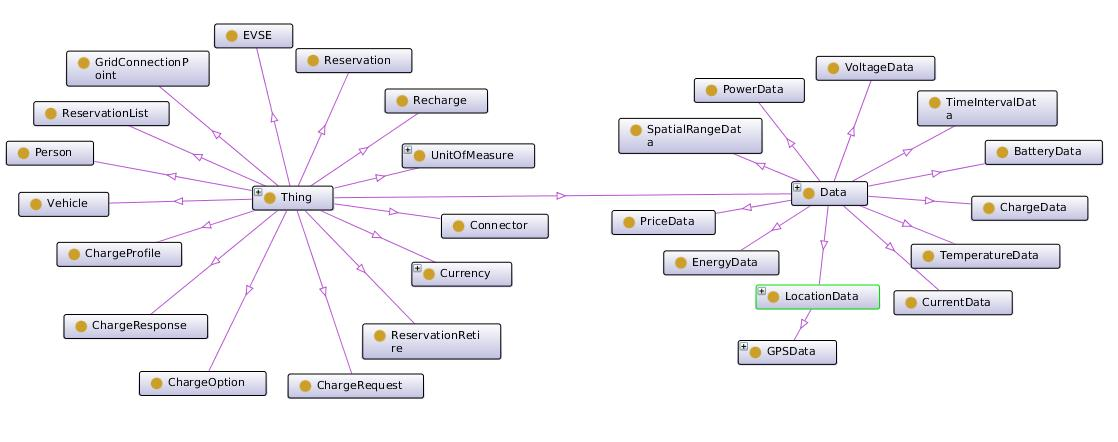
\includegraphics[width=1.0\textwidth]{assets/ontology-pro.jpg}
	\caption{Rappresentazione grafica delle classi dell'ontologia}
	\label{fig:ioe-ontology}
\end{figure}

\subsection{Modifiche apportate all'ontologia}

La versione dell'ontologia su cui ho iniziato a lavorare era la 1.5.4 alla quale sono seguiti 10 successivi rilasci fino all'attuale release 1.6.2. Le modifiche più importanti hanno riguardato il supporto di un nuovo protocollo di prenotazione delle ricariche oltre a operazioni varie operazioni di refactoring e correzione di incongruenze.

\subsubsection{Il concetto di Utente}\label{subsubsec:person}

Inizialmente il concetto di utente non era previsto nell'ontologia in quanto non trovava nessuna applicazione pratica.
L'entità che interagiva con la Grid era il veicolo e non l'utente. Questo approccio evidenzia i suoi limiti nel caso in cui un utente possieda più veicoli e voglia monitorarne contemporaneamente le ricariche effettuate o le prenotazioni pendenti. Inoltre anche dal punto di vista dei fornitori di corrente elettrica può essere utile una visione a livello di utente per semplificare le operazioni di fatturazione. Successivamente è stata introdotta la necessità di autenticare gli utenti per poter cifrare le comunicazioni con il SIB. 

È stata quindi introdotta la classe \code{ioe:Person}. Seppur esistano già delle ontologie con classi che rappresentative di questo concetto, si è ritenuto più semplice crearne uno nostro. Sviluppi futuri potrebbero legare questo concetto ad uno già esistente per rendere più semplice l'interoperabilità tra sistemi diversi. La classe presenta le seguenti proprietà:

\begin{itemize}
	\item \code{ioe:hasName}: Nome e Cognome dell'utente in formato stringa. Attualmente è irrilevante avere una separazione dei due. 
	\item \code{ioe:hasUserIdentifier}: codice che identifica univocamente l'utente.
	\item \code{ioe:hasVehicle}: proprietà associa a un utente uno o più veicoli.
\end{itemize}

\noindent
Come si può vedere attualmente l'utente è modellato in modo molto primitivo. Sono state infatti incluse solo le proprietà strettamente necessarie al nostro ambito di interesse. 

\subsubsection{Il concetto di Veicolo}\label{subsubsec:vehicle}

Nel vecchio modello ontologico il concetto di veicolo, in quanto non essenziale, non veniva particolarmente enfatizzato. Nella ultime versioni dell'ontologia ho aggiunto al veicolo alcune proprietà per soddisfare all'esigenza di distinguere le diverse possibili provenienze dei veicoli. Infatti i veicoli vengono inseriti nel SIB dal simulatore e possono anche essere reali come nel caso del Fiat Daily provato al CRF (App. \ref{app:crf}).

Il veicolo è attualmente definito dalle seguenti proprietà:

\begin{itemize}
	\item \code{ioe:hasManufacturer}: Casa automobilistica che produce il veicolo.
	\item \code{ioe:hasModel}: mdello del veicolo.
	\item \code{ioe:hasGPSData}: la proprietà punta ad un istanza di \code{ioe:GPSData} che a sua volta contiene le informazioni di latitudine e longitudine.
	\item \code{ioe:hasBatteryData}: la proprietà punta ad un istanza di \\ \code{ioe:BatteryData} contenente i dati della batteria.
	\item \code{ioe:hasIdentificationData}: identificativo del veicolo attualmente non utilizzato a favore della più semplice proprietà \code{ioe:hasName}.
\end{itemize}

\subsubsection{Il concetto di Ricarica}

Nella prime versioni dell'ontologia non esisteva nulla che indicasse il concetto di ``ricarica avvenuta'', molto utile per le statistiche lato utente (es: quanto si è speso in un mese per ricaricare il veicolo) e lato Grid (es: quanta energia è stata erogata e quali sono stati gli introiti). Questo perché i tempi previsti dalla prenotazione possono differire sensibilmente da quelli reali: basti pensare a una persona che arriva in ritardo a ricaricare il veicolo o che lascia la colonnina in anticipo. 

È stata quindi introdotta la classe \code{ioe:Recharge}. Si noti che le proprietà di seguito elencate sono state decise di comune accordo con un altro partner del progetto IoE, la spagnola AICIA, allo scopo di eseguire una demo congiunta in cui dimostrare l'interoperabilità tra la nostra piattaforma e quella sviluppata da loro.

\begin{itemize}
	\item \code{ioe:hasDate}: data e ora in cui è avvenuta la ricarica.
	\item \code{ioe:hasUser}: utente che ha effettuato la ricarica, da cui si evidenzia la necessità di inserire la classe \code{ioe:Person} (\ref{subsubsec:person}).
	\item \code{ioe:hasRechargeTime}: il tempo necessario ad effettuare la ricarica.
	\item \code{ioe:hasConsumption}: la quantità di corrente impiegata per effettuare la ricarica.
\end{itemize}

\subsubsection{Il Vecchio Protocollo di Prenotazione}\label{subsubsec:old-proto}

Il protocollo di prenotazione iniziale era in stato embrionale e serviva a scopo esemplificativo per dimostrare la fattibilità del progetto. I parametri previsti per la richiesta di ricarica, ovvero le proprietà della classe \code{ioe:ChargeRequest} erano:

\begin{itemize}
	\item \code{ioe:hasPreferredTime}: la data in cui l'utente desidera effettuare la ricarica.
	\item \code{ioe:hasPosition}: la posizione da cui si sta eseguendo la richiesta.
	\item \code{ioe:hasRequestedEnergy}: la quantità di carica richiesta. 
	\item \code{ioe:hasRequestingVehicle}: il veicolo che richiede la ricarica.
	\item \code{ioe:hasChargeResponse}: la risposta fornita dal sistema.
\end{itemize}

\noindent
In seguito ad alcune problematiche verificatesi durante le simulazioni è stato necessario aggiornare il protocollo, all'epoca ancora in fase embrionale.
Al di la della mancanza del concetto di utente, l'assenza di range nei campi \code{ioe:hasPreferredTime} e \code{ioe:hasPosition} poteva portare ad un eccessiva ridondanza delle risposte con conseguenti insostenibilità nei tempi e nelle entità del traffico di dati particolarmente in caso di utilizzo di smartphone agganciati alla rete tramite connettività mobile.

\subsubsection{Il nuovo Protocollo di prenotazione}\label{subsubsec:chargerequest}

In seguito ai problemi messi in luce nel paragrafo precedente (\ref{subsubsec:old-proto}) si è deciso di sviluppare un nuovo protocollo di prenotazione che prendesse in considerazione i nuovi requisiti funzionali (Fig. \ref{fig:res-sec}).

La classe è \code{ioe:ChargeRequest} è stata quindi ridefinita con le seguenti proprietà:

\begin{itemize}
	\item \code{ioe:hasRequestingUser}: utente che richiede la ricarica. Malgrado si possa risalire all'utente tramite il veicolo è stato comunque inserita la proprietà al fine di semplificare le query SPARQL.
	\item \code{ioe:hasSpatialRange}: area nella quale si vuole eseguire la ricarica. Il punto centrale di quest'area non corrisponde necessariamente con la posizione dell'utente. Come vedremo nella sezione relativa all'applicazione mobile (\ref{chap:mobile-app}) l'area di prenotazione può essere scelta arbitrariamente sulla mappa.
	\item \code{ioe:hasTimeInterval}: il range temporale all'interno del quale si è disposti ad eseguire la ricarica. Può anche essere molto superiore al tempo necessario per la ricarica nel caso in cui non ci siano particolari requisiti di tempo.
	\item \code{ioe:hasRequestingVehicle}: il veicolo per cui si richiede la ricarica. Non differisce rispetto al vecchio protocollo.
	\item \code{ioe:hasRequestedEnergy}: la quantità di carica richiesta. Non differisce rispetto al vecchio protocollo.
\end{itemize}

\noindent
Per quanto migliorato il protocollo è ancora incompleto ed in quanto tale è ancora suscettibile di ulteriori significative migliorie. Ora ad es. non è possibile specificare la volontà dell'utente di essere più flessibile riguardo alla quantità di carica richiesta e nemmeno, nel caso sia richiesto dalla Grid, se fosse disposto a cedere parte della sua carica.
\\ \\
Oltre alla richiesta è stata modificata anche la risposta. Alla classe \code{ioe: ChargeResponse} è stata aggiunta la proprietà \code{ioe:hasRelatedRequest} per semplificare le query SPARQL. Anche le opzioni di ricarica contenute nella risposta sono state modificate non solo per farle aderire ai nuovi requisiti funzionali ma anche per semplificare le query SPARQL.

Di seguito verranno esposte le proprietà della classe \code{ioe:ChargeOption}. Dalla vecchia definizione è stata rimossa la proprietà \code{ioe:hasChargeProfile}. Le proprietà ereditate dalla vecchia ontologia verranno opportunamente segnalate.

\begin{itemize}
	\item \code{ioe:optionHasEVSE}: EVSE presso il quale avverrà la ricarica (ereditata).
	\item \code{ioe:hasTimeInterval}: è un istanza della classe \code{ioe:TimeIntervalData}. Specifica il tempo necessario a ricaricarsi calcolato sulla base di energia richiesta e di potenza della potenza colonnina. La proprietà era presente anche nella vecchia definizione con i tempi indicati con le date in formato gg/mm/aaaa sostituita con gli attuali millisecondi (passati dalla mezzanotte del 1 Gennaio 1970 UTC) con le proprietà \code{ioe:hasFromTimeMillisec} e \code{ioe:hasToTimeMillisec}.
	\item \code{ioe:hasRequestingVehicle}: il veicolo per cui è stata effettuata la richiesta. (ereditata)
	\item \code{ioe:hasRequestingUser}:l'utente che ha effettuato la richiesta.
	\item \code{ioe:hasGridConnectionPoint}: il GCP presso cui avverrà la ricarica. Malgrado vi si possa accedere tramite l'EVSE è stato inserito per semplificare le query SPARQL.
	\item \code{ioe:hasTotalPrice}: prezzo totale della ricarica.
	\item \code{ioe:hasGcpPosition}: posizione del GCP. Anche questa proprietà è stata aggiunta per semplificare le query SPARQL.
\end{itemize}

\begin{figure}
	\centering
	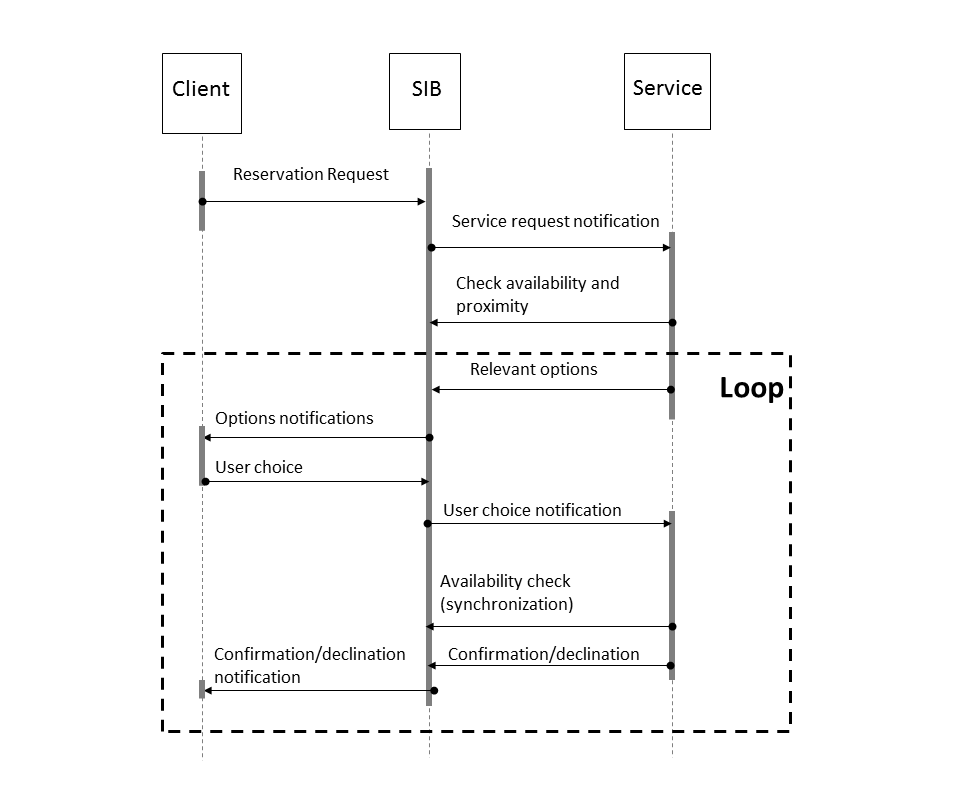
\includegraphics[width=1.0\textwidth]{assets/reservation-seq-diagram.png}
	\caption{Sequence diagram che schematizza il protocollo di richiesta}
	\label{fig:res-sec}
\end{figure}

\subsubsection{Rimozione informazioni Hardcoded}

Fino alla versione 1.5.11 dell'ontologia le informazioni relative ai GCP erano hardcoded nell'ontologia, scelta che all'inizio del progetto è stata dettata del poco tempo. Successivamente questo approccio si è rivelato fortemente limitante poiché la modifica dell'ontologia è un operazione abbastanza tediosa e sopratutto poco flessibile. 

Per di risolvere questo problema ho deciso di rimuovere questi dati dall'ontologia e inserirli all'interno di un file XML che viene caricato dal \emph{City Service} (Sez. \ref{subsubsec:city-init}) e dal simulatore (Sez. \ref{chap:sim}) in fase di inizializzazione.

Grazie a questo approccio è diventato relativamente semplice impostare uno scenario del tutto diverso da quello previsto inizialmente dal progetto.

\section{I Semantic Information Broker}

I SIB sono alla base dell'infrastruttura semantica che caratterizza il progetto. I componenti del sistema (dal servizio cittadino, allo smartphone, all'EVSE ecc\dots) comunicano e rendono permanenti le informazioni grazie ad essi. L'architettura rimane sostanzialmente invariata da quella presentata da Federico Montori (\cite{montori2012}) nel suo progetto di tesi. Verrà comunque esposta al fine di comprendere il resto della trattazione e verranno evidenziate le variazioni apportate alla soluzione iniziale.

L'architettura proposta prevede 2 SIB: il \emph{City SIB} e il \emph{Dash SIB} e una sua schematizzazione è rappresentata in Fig. \ref{fig:proj-sib-arch}.

\subsection{City SIB}\label{subsec:city-sib}

Il \emph{City SIB} è il SIB cittadino. Al suo interno vengono immagazzinate tutte le informazioni utili a caratterizzare uno scenario di mobilità elettrica veicolare. Si usa inoltre come interfaccia di scambio dati tra il \emph{City Service} e gli agenti esterni. È infatti nel emph{City SIB} che vengono scritti i messaggi che compongono i protocolli i quali vengono cancellati una volta terminati. L'area di copertura di tale SIB e di conseguenza del \emph{City Service} è definita dalla classe dell'ontologia \code{ioe:Zone} anche se attualmente non viene utilizzata poiché gli scenari proposti prendono in considerazione una città alla volta.

Per di poter rispondere alle richieste di prenotazione degli utenti il \emph{City Service} contiene le informazioni relative a tutte le colonnine della zona che ricopre. Possiede inoltre le informazioni relative agli utenti e ai veicoli di competenza. Non contiene le informazioni relative alla batteria, contenute nel \emph{Dash SIB} (\ref{subsec:dash-sib}). Nell'architettura proposta nel progetto precedente gli utenti non erano previsti (\ref{subsubsec:person}) per cui le informazioni relative ai veicoli si trovavano esclusivamente nella \emph{Dash SIB}.

L'inizializzazione del \emph{City SIB}, contrariamente a quanto avveniva in precedenza, viene eseguita dal servizio cittadino che inoltre il servizio cittadino si occupa di caricare le informazioni dei GCP da un file XML e di inserirle nel SIB (Sez. \ref{subsubsec:city-init}).

\subsection{Dash SIB}\label{subsec:dash-sib}

Il \emph{Dash SIB} è  un SIB che dovrebbe essere integrato a bordo di ogni veicolo. Il suo scopo è tenere costantemente traccia dei parametri che caratterizzano posizione, stato della batteria e tutti gli altri parametri variabili che caratterizzano un veicolo. Per collegare questi dati a un veicolo la tripla che descrive un istanza di \code{ioe:Vehicle} viene ripetuta anche su questo SIB. 

Inizialmente si pensava che questo SIB sarebbe stato eliminato in un contesto reale in quanto i dati in esso contenuti sarebbero stati letti direttamente dal veicolo. Si è invece deciso di mantenerlo con la funzione di interfaccia comune per l'interrogazione dei dati. Ovvero le applicazioni che utilizzano i dati del veicolo, come ad esempio l'applicazione mobile, dovrebbero essere indifferenti alla sorgente dei dati (es: Veicolo Reale, Veicolo Simulato). Compito del programmatore è implementare un adattatore che scrive i dati in provenienti dalle varie fonti sul \emph{Dash SIB}. Come vedremo più avanti (Cap. \ref{chap:mobile-app} e \ref{chap:sim}) grazie a questa tecnica si può controllare dallo smartphone un veicolo presente nel simulatore tenendone monitorati tutti i parametri. I veicoli del simulatore scrivono tutti sullo stesso \emph{Dash SIB} in quanto sarebbe computazionalmente proibitivo e del tutto inutile fare altrimenti.

Poiché attualmente non esistono veicoli dotati di un SIB, in fase di test su veicolo reale (App. \ref{app:crf}) è stato necessario dotarsi di un computer a bordo che contenesse il \emph{Dash SIB} dal quale l'applicazione mobile prelevava i dati.

\begin{figure}[H]
	\centering
	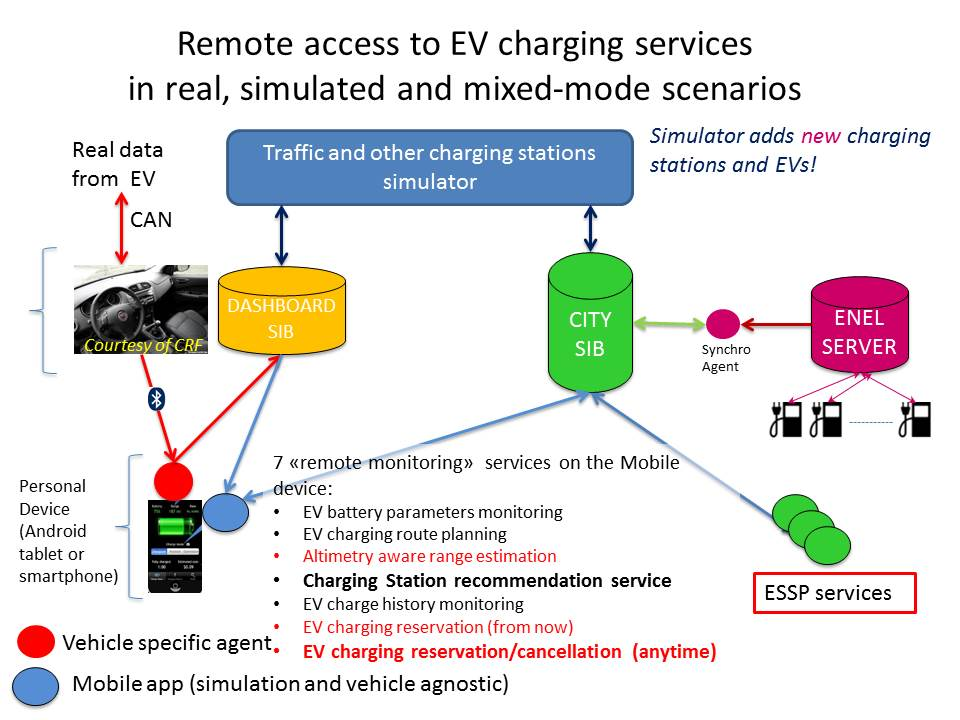
\includegraphics[width=1.0\textwidth]{assets/software-architecture.jpg}
	\caption{Architettura proposta per il progetto}
	\label{fig:proj-sib-arch}
\end{figure}

\section{La libreria IoE}\label{subsec:ioe-lib}

Implementa la logica applicativa ovvero il nucleo operativo del nostro strato di servizi. È la base per qualunque applicazione che intenda interfacciarsi con il sistema in modo semplice ed efficace. Viene infatti sfruttata sia dal \emph{City Service} che dall'applicazione mobile, da me sviluppati. Viene inoltre utilizzata da un visualizzatore di ricariche, nato da un progetto parallelo a questo, del cui sviluppo si è occupata una studentessa di Ingegneria.

\subsection{Connessione al SIB}

La connessione al \emph{SIB} è implementata da una libreria Java (JavaKPI), sviluppata da ARCES, che fa uso del protocollo SSAP. Ho creato un wrapper di questa libreria che ne semplifica l'utilizzo e aggiunge alcune funzionalità: si trova nel package \code{it.unibo.ioe.sib}.

\subsubsection{RdfTriple}

La libreria JavaKPI rappresenta le triple RDF come vettore di Stringhe di 5 elementi (\code{Vector<String>}): soggetto, predicato, oggetto, tipo soggetto, tipo oggetto (dove con tipo si intende o un URI, ovvero un'altra istanza di classe dell'ontologia, oppure un letterale ovvero un dato diretto). 
Per semplificare la gestione delle triple RDF, che sono l'entità di base del SIB, ho creato la classe \code{RdfTriple} che possiede gli attributi \code{subject}, \code{predicate}, \code{object}, \code{subjectType}, \code{objectType} e i corrispettivi \code{getter} e \code{setter}.

\subsubsection{KpConnector}

La maggior parte delle operazioni che si possono eseguire con la libreria JavaKPI richiedono due passaggi: l'invio del comando e il parsing della risposta. Questo perché ogni operazione di interazione con il SIB avviene tramite messaggi XML conformi al protocollo SSAP. La libreria genera automaticamente il messaggio da inviare alla SIB ma lascia al programmatore l'onere di effettuare il parsing della risposta. Ho quindi mappato tutte le operazioni di interazione con la SIB all'interno della classe \code{KpConnector}.

La classe \code{KpConnector} svolge le operazioni di parsing anche sui messaggi di risposta. Anzichè i vettori di stringhe ho utilizzato istanze della classe \code{RdfTriple}. Inoltre ho sostituito le liste di triple (es: inserimento multiplo di triple, risultati di query SPARQL implementati con \code{Vector<Vector<String>>}) con liste di oggetti di tipo \code{RdfTriple} (\code{List<RdfTriple>}). \code{RdfParser} è la classe che converte i tipi di dato usati dalla libreria \code{JavaKPI} nei tipi usati dal wrapper che ho implementato.

\subsubsection{KpFactory}

La classe \code{KpConnector} necessita di indirizzo, porta e nome del SIB a cui ci si vuole connettere ai fini dell'utilizzo più generico possibile. Nel nostro caso però le connessioni avvengono sempre verso gli stessi due SIB (\emph{City} e \emph{Dash}), quindi ho creato una classe factory (\code{KpFactory}) che, noti i parametri di connessione necessari, crea due istanze di \code{KpConnector}, una per il \emph{City SIB} e una per il \emph{Dash SIB}. Quando è necessario connettersi ai SIB il factory restituisce gli oggetti precedentemente creati evitando quindi la creazione di istanze di oggetti inutili. Non essendo la libreria JavaKPI \emph{thread-safe} viene comunque data la possibilità di creare nuove istanze nel caso si lavori in ambienti multi-thread. Questo aspetto verrà approfondito più avanti dove vedremo come, tramite la tecnica dei pool di oggetti, si può risparmiare il tempo necessario a creare nuove istanze.

%http://sourceforge.net/projects/smartm3-javakpi/

\subsection{Entities}

Ogni classe dell'ontologia è stata mappata con una rispettiva classe Java (Entity) nel package \code{it.unibo.ioe.entity}. Per questa scelta architetturale mi sono ispirato all'ORM (Object Relational Mapping), tecnica di programmazione che favorisce l'integrazione di sistemi software aderenti al paradigma della programmazione orientata agli oggetti con sistemi RDBMS (Relational Database Management System). %http://it.wikipedia.org/wiki/Object-relational_mapping

\subsubsection{Mapping} 

Ho realizzato un mapping molto semplice che tiene conto delle sole proprietà necessarie nello strato di servizi 
 tralasciando alcuni dettagli, come l'unità di misura, che attualmente, malgrado siano previsti nell'ontologia, vengono dati per scontati a livello applicativo.
Le proprietà delle classi che hanno come oggetto un letterale sono state mappate con tipi primitivi Java (\code{int},  \code{double}, \code{String} ecc..). Le proprietà che invece come oggetto hanno un'altra classe sono rappresentate come attributo avente come tipo l'Entity che corrisponde alla classe. 

\subsubsection{Serializzazione} 

Alcune Entity sono state opportunamente annotate per poterle serializzate in XML tramite la tecnologia \code{JAXB}. Questo è risultato necessario nel caso dei GCP che vengono caricati da un file XML dal \emph{City Service} che poi li inserisce nel SIB. Ogni classe inoltre implementa l'interfaccia \code{java.io.Serializable} per consentire il passaggio delle Entity tra le varie \code{Activity} dell'applicazione mobile.

\paragraph{Esempio}

La proprietà dell'ontologia \code{ioe:hasEVSE} ha come dominio \\ \code{ioe:GridConnectionPoint} e come codominio \code{ioe:EVSE}. Inoltre tutte le classi dell'ontologia hanno al proprietà \code{ioe:hasName}.

Questo si traduce nell'Entity mostrato nel Lst. \ref{lst:entity}

\begin{java}[caption={Entity di esempio},label={lst:entity}]
@XmlRootElement(name = "GCP")
@XmlAccessorType(XmlAccessType.FIELD)
public class GCP implements Serializable {
	@XmlTransient
	private String URI;
	private String gcpName;
	@XmlElement(name = "EVSE")
	private List<EVSE> evseList;
	/* other properties*/
	/* getter & setter*/	
}
\end{java}

\subsection{Controller}

I \code{Controller} sono le classi delegate ad eseguire le operazioni \code{CRUD} (create, read, delete, update) con il SIB e si trovano nel package \code{it.unibo.ioe .controller}. Ne esiste uno per ogni Entity. Ogni \code{Controller} possiede un'istanza di \code{KpConnector} che realizza la comunicazione con il SIB. 

\begin{description}
	\item \textbf{Lettura} Le operazioni di lettura si eseguono con una query SPARQL che preleva dal SIB le informazioni necessarie per poi inserirle in una nuova istanza di Entity la quale viene restituita all'utente.

	\item \textbf{Scrittura} Le operazioni di scrittura ricavano una lista di triple RDF a partire da un istanza di Entity. La lista di triple viene poi convertita in una \emph{SPARQL insert} per ridurre i dati inviati al SIB. L'operazione di conversione è eseguita da una funzione della classe \code{SibUtil}. Questa tecnica si rivela particolarmente utile quando si usa la libreria da un dispositivo mobile connesso a internet tramite rete cellulare (es: EDGE, GPRS, HSDPA ecc\dots). Si noti che tutte le Entity possiedono un campo \code{URI} che viene valorizzato nell'operazione di inserzione con l'URI assegnato all'istanza che si sta per scrivere sul SIB. 

	\item \textbf{Aggiornamento} Le operazioni di aggiornamento ricavano i dati aggiornati tramite una query SPARQL e andranno a sostituire quelli obsoleti all'interno di un istanza di Entity

	\item \textbf{Rimozione} Le operazioni di rimozione lato \emph{City Service} sono eseguite direttamente tramite \emph{SPARQL delete}. Le operazioni di rimozione all'esterno (es. applicazione mobile) per motivi di sicurezza sono invece eseguite tramite richiesta al servizio cittadino il quale si occupa di effettuare la rimozione vera e propria.
\end{description}
	  
\chapter{Servizio Cittadino}

Il servizio cittadino (\emph{City Service}) è il cuore dell'architettura software e, al fine di supportare le interazioni tra gli EV e la Smart Grid. Lo scambio di informazioni avviene tramite un SIB cittadino e la struttura dei messaggi è definita all'interno dell'Ontologia. 

\section{Architettura}

Il principio di base con cui ho progettato il \emph{City Service} è la modularità e riusabilità. Ho quindi creato una libreria, \code{ioe_lib}, condivisa tra il servizio cittadino e l'applicazione mobile. Essa fornisce i servizi di base di accesso al \emph{SIB}, nonchè un approccio \emph{Object Oriented} ai dati in essa contenuti. Ho infatti implementato, per ogni classe presente nell'ontologia, una corrispettiva classe Entity Java e un \code{Controller} che incapsula la logica di lettura scrittura e aggiornamento dei dati nella \emph{SIB}. Questa scelta progettuale si rifà ai principi di Ingegneria del Software \emph{High Cohesion} e \emph{Low Coupling} \cite{larcab2005}

\section{La comunicazione con il City Service}\label{sec:protocol}

In questa sezione analizzeremo in dettaglio come avviene la comunicazione da e verso il servizio cittadino. Per ogni operazione esiste un protocollo basato su scambi di messaggi la quale struttura è definita attraverso classi dell'ontologia. Attualmente le uniche operazioni supportate sono la richiesta di prenotazione e la richiesta di ritiro di prenotazione.

Lo scambio dei messaggi è implementato tramite il meccanismo delle \code{Subscription} messo a disposizione dal SIB. Questo comporta che i messaggi vengono scritti sul \emph{SIB} cittadino il quale manda una notifica al \emph{KP} che era sottoscritto a quella particolare modifica. Questo rende il protocollo di comunicazione asincrono.


\subsection{Protocollo di richiesta di prenotazione}

Qui verranno descritti tutti i passaggi necessari al completamento del protocollo di Richiesta di Prenotazione, in particolare quali messaggi vengono scambiati. Il fine della Prenotazione è avere la certezza che quando andremo a caricarci troveremo l'EVSE libero. Come già detto in precedenza, i tempi di ricarica per i veicoli elettrici possono essere molto lunghi. È quindi necessario dare all'utente la sicurezza che potrà ricaricare il suo veicolo senza il rischio di terminare la batteria.

\begin{enumerate}[label=\textbf{\arabic*}]
	\item \textbf{Richiesta di Prenotazione}: Quando l'utente necessita di fare una ricarica inserisce una richiesta nel SIB. La richiesta è descritta dalla classe dell'ontologia \code{ioe:ChargeRequest}.
	\item \textbf{Risposta da parte del City Service}: Il servizio cittadino è sottoscritto all'inserimento di nuove istanze di \code{ioe:ChargeRequest}. Quindi, quando viene inserita la richiesta, arriva una notifica che ne contiene l'URI dal quale si possono ricavare tutti i parametri che la compongono. A questo punto viene creata una lista di opzioni di ricarica conformi alla richiesta dell'utente compatibilmente con la disponibilità degli EVSE. Le opzioni di ricarica sono classi di tipo \code{ioe:ChargeOption} e vengono inserite dentro a una classe di tipo \code{ioe:ChargeResponse}.
	\item \label{item:confirmByUser} \textbf{Conferma da parte dell'utente}: L'utente che è sottoscritto all'inserimento di nuove istanze della classe  \code{ioe:ChargeResponse} viene notificato quando il \emph{City Service} inserisce la risposta. Le opzioni di ricarica vengono analizzate dall'utente il quale sceglie quella che più si addice alle sue esigenze. La scelta viene notificata al sistema tramite inserimento di una tripla così formata: \code{[ioe:chargeOptURI ioe:confirmByUser "true"]} presupponendo che \code{ioe:chargeOptURI} sia un istanza di \code{ioe:ChargeOption}.
	\item \textbf{Conferma da parte del City Service)}: Il servizio cittadino è iscritto all'inserimento di triple che come predicato hanno \code{ioe:confirmByUser} e quindi verifica se l'opzione selezionata è ancora disponibile in tal caso inserisce una tripla siffatta:
	\\ \code{[ioe:chargeOptURI ioe:confirmBySystem "true"]}. 
	\item \textbf{Acknowledgment da parte dell'utente}: L'utente riceve la notifica della conferma da parte di \emph{City Service}. Se l'opzione è confermata allora invia una tripla di Acknowledgment \code{[ioe:userURI ioe:ackByUser "true"]}. Altrimenti può provare con un altra opzione e il protocollo riprende dal punto ~\ref{item:confirmByUser}
	\item \textbf{Creazione Prenotazione}: Quando il \emph{City Service} riceve l'acknowledgment dall'utente "blocca" l'EVSE nella finestra di tempo richiesta creando un istanza della classe {ioe:Reservation}. Inoltre cancella dal SIB tutte le triple necessarie allo svolgimento del protocollo che  , una volta terminato, diventano inutili.
\end{enumerate}

\section{Il Protocollo di rimozione di una prenotazione}

Una volta completata la procedura di prenotazione l'EVSE è diventa inagibile nell'orario richiesto dall'utente. Nel caso in cui un utente voglia ritirare la prenotazione deve mandare una richiesta al \emph{City Service}. Attualmente il servizio cittadino rimuove semplicemente dal SIB i dati relativi alla prenotazione rendendo nuovamente disponibile la ricarica. In futuro il servizio potrà stabilire, in base a regole dettate dai gestori della rete elettrica, se accettare o meno la richiesta ed eventualmente accreditare una penale all'utente.

Il Protocollo si basa su cambio di messaggi proprio come nel caso precedente.

\begin{enumerate}
	\item \textbf{Richiesta ritiro Prenotazione}: L'utente inserisce nel SIB cittadino un istanza della classe \code{ioe:ReservationRetire} 
	\item \textbf{Ritiro della Prenotazione}: Il \emph{City Service}, che ovviamente era sottoscritto alla creazione di nuove istanze di \code{ioe:ReservationRetire}, provvede a rimuovere dal SIB le triple relative alla Prenotazione.
	\item \textbf{Notifica avvenuta cancellazione}: Attualmente l'utente come unico modo per sapere dell'avvenuta cancellazione deve sottoscriversi ai cambiamenti dell'URI della Prenotazione che sta cancellando.
\end{enumerate}

\section{Implementazione}\label{sec:impl}

In questa sezione discuteremo i dettagli implementativi del \emph{City Service}, dalle tecnologie usate alle scelte Architetturali. Principalmente il serbizio cittadino deve essere altamente performante in quanto, una vota a regime, dovrebbe poter soddisfare le richieste di centinaia di utenti se non migliaia. Contemporaneamente bisogna preoccuparsi del fatto che l'alto parallelismo non intacchi l'integrità dei dati residenti sul SIB cittadino evitando, ad esempio, che due persone che fanno una prenotazione nello stesso momento, nello stesso EVSE, alla stessa ora non riescano entrambe a completare la procedura di prenotazione. 

Il servizio è scritto interamente in Java il che lo rende multi piattaforma, facile da debuggare, e sopratutto permette di usare utilità estremamente versatili riguardanti il multi-threading messe a disposizione dal linguaggio. Inoltre permette di accedere alla moltitudine di librerie scritte per questo linguaggio per i più disparati propositi. Tra queste troviamo (log4j), un robusto quanto versatile sistema di logging, che permette di tenere costantemente sotto controllo l'esecuzione del servizio con vari gradi di granularità del log.

Al fine di rendere il servizio più performante possibile sono state adottate tecniche di programmazione quali: pool di oggetti, pool di thread, e caching delle risorse.


\subsection{Pool Di Oggetti}

Per effettuare le connessioni al SIB cittadino è necessario istanziare oggetti di tipo \code{KpConnector}, inoltre, per effettuare il parsing delle risposte alle sottoscrizioni sono necessari oggetti di tipo \code{SSAP_XMLTools} che sono forniti dalla libreria \code{JavaKPI}. Come è stato detto nella sezione ~\ref{sec:impl} il \emph{City Service} deve supportare connessioni multiple simultanee, ognuna delle quali dialoga con il SIB. Dal momento che la libreria {JavaKPI} non è thread-safe e nemmeno il wrapper che ho creato io lo è, è necessario istanziare un oggetto \code{KpConnector} per ogni connessione insieme a uno di tipo \code{SSAP_XMLTools} per parsare i risultati delle sottoscrizioni.

Per evitare che all'avvio di ogni connessione venisse creato un oggetto \code{KpConnector}, che comunque è un oggetto "pesante", ho deciso di usare la tecnica dei pool di oggetti. La tecnica consiste nel creare un numero sufficienti di oggetti all'inizio dell'applicazione e quando si necessita di usarne uno lo si chiede al pool il quale lo fornisce al tempo di una chiamata a metodo. Una volta terminato di utilizzare l'oggetto lo si restituisce al pool il quale poi potrà a sua volta cederlo ad un altro richiedente.
In questo modo si evita che ogni volta che viene fatta una richiesta al \emph{City Service} ci sia il delay necessario a instanziare una connessione con il SIB.

C'è da dire che vista le ottimizzazioni delle moderne \emph{Java Virtual Machine} e del \emph{Garbage Collector} per quanto riguarda gli oggetti con breve durata questa tecnica può rischiare di abbassare le performance anziché aumentarle \cite{torok2011}. Rimane comunque vantaggiosa nel caso di oggetti la quale creazione può essere abbastanza onerosa come per le connessioni ai database o alla rete.

Il cuore di questo sistema è la classe \code{ObjectPool<T>} (\cite{objectpool}) che troviamo nel package \code{it.unibo.cityservice.pool} che rappresenta un pool di oggeti di tipo \code{T}. Questa classe contiene un metodo astratto \code{createObject()} che va implementato nelle sottoclassi mettendoci dentro la logica di creazione dell'oggetto di cui volgiamo creare il pool.

Nel mio caso ho creato \code{XmlToolsPool} e \code{CitySibPool} e a titolo esemplificativo mostrerò l'implementazione del primo:

\begin{java}[caption={Implementazione di ObjectPool},label={lst:objectPool}]
public class XmlToolsPool extends ObjectPool<SSAP_XMLTools>{
	
	public XmlToolsPool(final int minIdle) {
		super(minIdle);
	}

	@Override
	protected SSAP_XMLTools createObject() {
		return new SSAP_XMLTools();
	}
}
\end{java}

\noindent
Come si può vedere è molto semplice creare un pool per un determinato tipo di dato. Una volta creato il pool, per interagire con esso, si usano i seguenti metodi:

\begin{itemize}
	\item \code{public T borrowObject()}: che preleva un oggetto dal pool.
	\item \code{public void returnObject(T object)}: che restituisce un oggetto al pool.
\end{itemize}

\subsection{Pool Di Thread}

Adesso che abbiamo visto come è che cos'è il meccanismo dei pool degli oggetti e perchè è stato utilizzato vediamo invece di capire cosa sono i pool di thread e quali problematiche vanno a risolvere.
La creazione di thread può creare problemi in termini di performance (in quanto la creazione e distruzione di questo oggetti è abbastanza onerosa), di controllare il numero del numero dei thread creati e infine di scalabilità (\cite{vetti2008}).

Pertanto è necessario ricorrere alle classi del package \code{java.util.concurrent} che implementano l'interfaccia \code{Executor}. In questo caso sono state poi utilizzate istanze dell'interfaccia \code{ExecutorService} che mette a disposizioni metodi volti a controllare il ciclo di vita del pool stesso.

L'inizializzazione degli \code{ExecutorService} avviene tramite l'invocazione di un metodo statico della classe \code{Executors} che specifica la dimensione del pool che si vuole creare. Quando invece si vuole assegnare un compito ad uno dei thread del pool si usa il metodo \code{execute} che prende in ingresso un istanza dell'interfaccia \code{Runnable}.

\begin{java}[caption={Creazione Pool di Thread},label={lst:threadPool}]
ExecutorService pool = Executors.newFixedThreadPool(30);
pool.execute(new Runnable() {
	@Override
	public void run() {
		System.out.println("hello world");
	}
});
\end{java}

\subsection{Il funzionamento del City Service}
 
Come visto nella sezione ~\ref{sec:protocol} il servizio cittadino deve gestire un gran numero di messaggi a ogni tipologia dei quali corrisponde una sottoscrizione al SIB cittadino. Inoltre per poter rispondere alle richieste degli utenti deve anche avere le informazioni relative a tutti gli EVSE.

\subsubsection{Inizializzazione}\label{subsubsec:city-init}

Il \textsc{City Service} all'avvio compie innumerevoli compiti. Contrariamente a quanto avveniva in precedenza, dove i GCP erano codificati nell'ontologia e l'ontologia stessa veniva caricata da un programma esterno, ho deciso di delegare le inizializzazioni al \textsc{City Service} col fine di semplificarne lo sviluppo. Infatti in precedenza ad ogni riavvio del servizio era necessario uccidere manualmente il SIB e riavviarlo per avere una situazione di partenza pulita. Il caricamento dell'ontologia avviene tramite una libreria da me sviluppata, \emph{OntologyLoader}, (App. ~\ref{app:ontology-loader}) che a sua volta si appoggia alle librerie Apache Jena (\cite{jena2011}). In ambito di produzione ovviamente il servizio cittadino non eliminerebbe i dati e nemmeno ricaricherebbe quelli già presenti.

Di seguito una lista dettagliata delle operazioni eseguite dal \textsc{City Service} in fase di inizializzazione:

\begin{itemize}
	\item \textbf{Lettura file di configurazione}: Cerca il file di configurazione \code{cityservice.properties} dal quale carica le informazioni del SIB cittadino, il nome dell'ontologia, il nome del file contenente i GCP.
	\item \textbf{Scrittura Ontologia}: L'ontologia viene scritta nel SIB cittadino
	\item \textbf{Caricamento Informazioni GCP}: Le informazioni di tutte le stazioni di ricarica presenti in città vengono caricate da un file xml. Le stesse informazioni vengono inserite nel SIB al fine di poterle condividee con le altre entità del sistema.
	\item \textbf{Creazione Pool}: Vengono creati i pool di thred e di oggetti.
	\item \label{item:subscr} \textbf{Sottoscrizioni}: Ci si sottoscrive alle informazioni su cui si vuole rimanere aggiornate. Sostanzialmente ci si assicura che arrivino le notifiche per i messaggi descritti nella sezione ~\ref{sec:protocol}:
	\begin{enumerate}
		\item Creazione di nuove istanze di \code{ioe:ChargeRequest}
		\item Inserimento di triple contenenti come predicato \code{ioe:confirmByUser}
		\item Inserimento di triple contenenti come predicato \code{ioe:ackByUser}
		\item Creazione di nuove istanze di \code{ioe:ReservationRetire}
	\end{enumerate}
\end{itemize}

\subsubsection{Gestione delle richieste}

Quando ci si sottoscrive a qualcosa nel SIB oltre a definire a cosa ci vogliamo sottoscrivere dobbiamo anche definire un \emph{handler} che verrà eseguito quando avverrà il cambiamento a cui siamo interessati. Come visto sopra, nella sezione ~\ref{sec:protocol}, di sottoscrizioni ne vengono fatte 4, per ognuna di esse viene definito lo stesso \emph{hanlder} il quale lancia un thread istanza della classe \code{RequestDispatcher}. Esso si occupa semplicemente di gestire la richiesta e di eseguire un altro thread, sempre contenuto in un pool, che la soddisfi.

\paragraph{Sessioni}

Per ottenere un ulteriore incremento di performace è stato introdotto il concetto di sessione. La sessione inizia al quando il \emph{City Service} riceve la richiesta e finisce quando riceve l'acknowledgment. Il fine della sessione è mantenere una cache dei dati che vengono scambiati al fine di risparmiare query SPARQL, che sono assai onerose in termini di performance, e di dare un limite temporale alle sessioni stesse. La classe che si occupa di gestire le sessioni è \code{SessionManager} mentre la sessione è rappresentata dalla classe \code{session}.

All'interno della sessione vengono salvate le seguenti informazioni:

\begin{itemize}
	\item \textbf{chargeRequest}: Un istanza dell'entity \code{ChargeRequest} ricevuta all'utente. 
	\item \textbf{chargeResponse}: Un istanza dell'entity \code{ChargeResponse} inviata all'utente. 
	\item \textbf{reservation}: Un istanza dell'entity \code{Reservation} creata in seguito alla conferma dell'utente.
	\item \textbf{startTime}: Il momento in cui inizia la sessione.
	\item \textbf{endTime}: Il momento in cui finisce la sessione che corrisponde all'arrivo dell'acknowledgment dell'utente.
\end{itemize}

\noindent
La classe \code{SessionManager} possiede un timer che a tempo prefissato lancia un thread che controlla le sessioni attive. Se una delle sessioni è attiva da molto tempo senza essere stata chiusa allora significa che probabilmente c'è stato un problema e quindi vengono rimossi dal SIB tutti i dati relativi alla sessione compresa la prenotazione.

\paragraph{Prenotazioni}

La gestione delle prenotazioni, una volta che sono state create e confermate dall'utente, è delegata alla classe \code{ReservationManager}. A suo interno vengono salvate in una cache le istanze di \code{Reservation} create. Quando arriva una nuova richiesta di prenotazione la verifica della disponibilità viene fatta su questa cache anziché sul SIB. Questo sempre al fine di ridurre gli accessi al database e il successivo parsing delle risposte.
Siccome l'uso di questa classe è altamente parallelo, ovvero possono accedervi molti thread contemporaneamente, viene utilizzata una mappa thread-safe messa a disposizione da java \code{ConcurrentHashMap}. Inoltre le operazioni di verifica di disponibilità delle prenotazioni vengono sono atomiche a livello di EVSE grazie a un lock per ognuno di essi. 

\paragraph{Thread}\label{par:thread}

Ci sono cinque classi diverse che implementano l'interfaccia \code{Runnable} ognuna delle quali ha il compito di gestire un determinato aspetto dei protocolli di richiesta. Ovviamente c'è un pool di esecuzione per ognuna di esse.

\begin{itemize}
	\item \code{RequestDispatcher}: È il thread che si occupa di smistare le richieste agli altri esecutori, viene eseguito ogni volta che arriva una notifica da una sottoscrizione. La decisione avviene in base all'id della sottoscrizione che viene assegnato in fase di inizializzazione ed immagazzinato all'interno di variabili globali. Il codice di questo del corpo di questo thread è mostrato nel listato ~\ref{lst:requestDispatcher} dive si nota chiaramente l'utilizzo del pool di oggetti e dei pool di thread nonché del \code{logger}. Questo approccio viene usato anche per gli altri thread con l'aggiunta del reperimento dei \code{KpConnector} dal relativo pool.
	\item \code{ChargeRequestHandler}: Viene eseguito quando un utente inserisce un istanza istanza di \code{ioe:ChargeRequest} nel SIB. Dalla sottoscrizione ne ricava l'URI e con l'apposito controller \code{ChargeRequestController} la trasforma in un Entity java istanza della classe \code{ChargeRequest}. I passaggi che dalla richiesta elaborano una risposta sono i seguenti:
	\begin{enumerate}
		\item Controllo di coerenza sulla richiesta. Se la richiesta non è valida allora viene inviata una risposta vuota. Altrimenti si procede con il resto delle operazioni.
		\item Viene creata un istanza di \code{Session} gestita dalla classe \code{SessionManager}.
		\item Scelta dei \emph{GCP} che si trovano nell'area scelta dall'utente tramite la libreria \code{UniboGeoTools}.
		\item Vengono ciclati tutti gli \emph{EVSE} appartenenti ai \emph{GCP} selezionati.
		\item Per ogni \emph{EVSE} vengono ricavati gli slot di tempo compatibili con la fascia oraria e la quantità di carica richieste dall'utente.
		\item Viene generata la risposta istanza dell'Entity \code{ChargeResponse}. Al fine di minimizzare lo scambio di dati attraverso la rete sopratutto per non penalizzare i dispositivi mobili, le richieste vengono filtrate. Vengono inviate le opzioni di ricarica provenienti dai 5 \emph{GCP} più vicini e ne vengono scelte al massimo 2 per ogni \emph{EVSE}
		\item La risposta viene trasformata inserita nel SIB tramite la classe \\ \code{ChargeResponseController}.
	\end{enumerate}
	\item \code{ConfirmByUserHandler}: Questo thread viene invocato quando l'utente scaglie un opzione di ricarica e semplicemente controlla che sia ancora disponibile. In tal caso crea la prenotazione in modo che nessun altro possa usare la colonnina nell'orario richiesto. Da notare che l'istanza di \code{ChargeOption} viene presa dalla cache contenuta nella sessione anziché tramite query SPARQL e che l'istanza di \code{Reservation} viene salvata nel gestore di prenotazioni \code{ReservationManager}.
	\item \code{AckByUserHandler}: Viene invocato quando l'utente conferma l'opzione di ricarica. A questo punto il protocollo può considerarsi terminato e quindi vengono eliminate tutte le informazioni ad esso relative dal SIB e la sessione associata. L'unica informazione che rimane è un istanza di \code{ioe:Reservation} nel SIB.
	\item \code{RetireReservationHandler}: Si occupa semplicemente di eliminare le istanze di \code{ioe:Reservation} dal SIB e le corrispettive informazioni nella cache contenuta in \code{ReservationManager}.
\end{itemize}

\begin{java}[caption={Corpo di RequestDispatcher},label={lst:requestDispatcher}]
SSAP_XMLTools xmlTools = xmlToolsPool.borrowObject();
String subscriptionID = xmlTools.getSubscriptionID(subscribeResult);

if (chargeRequestSubId.equals(subscriptionID)) {
	chargeRequestExecutor.execute(new ChargeRequestHandler(subscribeResult));
} else if (confirmByUserSubId.equals(subscriptionID)) {
	confirmByUserExecutr.execute(new ConfirmByUserHandler(subscribeResult));
} else if (ackByUserSubId.equals(subscriptionID)) {
	ackByUserExecutor.execute(new AckByUserHandler(subscribeResult));
} else if (retireReservationSubId.equals(subscriptionID)) {
	retireReservationExecutor.execute(new RetireReservationHandler(subscribeResult));
} else {
	logger.error("Unexpected subscription id: " + subscriptionID);
}

xmlToolsPool.returnObject(xmlTools);
\end{java}	


\section{Testing}

Aspetto fondamentale che ha caratterizzato lo sviluppo del \emph{City Service} è stata l'integrazione con test di unità che ne hanno assicurato la continuità di funzionamento durante le fasi di modifica e sviluppo.

Il framework utilizzato per eseguire il testing è \code{junit4}, un ottima libreria Java che tramite il meccanismo delle annotazioni permette di scrivere ed eseguire i test i maniera semplice ed efficace.

I test sono stati determinanti non solo per assicurare la stabilità del codice ma anche per testare le performance del sistema, soprattutto del SIB. 

\subsection{Test Protocolli}

Per testare i protocolli ho implementato un thread che svolgesse tutte lo operazioni necessarie per completare una richiesta di prenotazione ed il ritiro della stessa. L'incapsulamento della logica del protocollo di richiesta all'interno di un thread permette di fatto l'esecuzione multipla di istanze di quest'ultimo simulando quindi l'interazione di molteplici utenti. La classe delegata a svolgere questo compito è \code{ioe:ChargeProtocolTest} nel packacge \code{it.unibo.ioe.cityservice.chargeprotocol} situato nella cartella di test. All'interno di questa classe si trova una inner-class, \code{ReservationProtocol} che implementa \code{Runnable} rendendo quindi possibile la sua esecuzione all'interno di un thread separato. 

Per simulare le attese dell'utente è stato usato il meccanismo dei lock. Ogni fase del protocollo ha un suo lock che viene acquisito subito dopo l'invio messaggio (List. ~\ref{lst:request-lock}) e viene rilasciato al momento dell'esecuzione l'handler associato alla sottoscrizione della risposta (List. ~\ref{lst:response-handler}).

\begin{java}[caption={Inserimento della \code{CargeRequest} e attesa della risposta},label={lst:request-lock}]
chargeRequestController.insertChargeRequest(request);
synchronized (chargeResponseLock) {
	try {
		chargeResponseLock.wait();
	} catch (InterruptedException ex) {
		logger.error(ex.getMessage(), ex);
	}
}
\end{java}

\begin{java}[caption={Handler associato al messaggio di risposta},label={lst:response-handler}]
String subscriptionID = xmlTools.getSubscriptionID(xml);
if (chargeResponseSubId.equals(subscriptionID)) {
		[...]
		chargeResponsesUri = subscriptionResult.get(0);
		synchronized (chargeResponseLock) {
			chargeResponseLock.notify();
		}
	}
}
\end{java}
\\
\noindent
L'opzione di ricarica viene scelta casualmente tra quelle fornite, nel caso in cui venisse confermata dal sistema il thread preleva la corrispondente istanza di \code{Reservation} creata e controlla che i parametri in essa contenuti siano coerenti con quelli dell'opzione scelta.\\
Tutti i dati scambiati dal protocollo vengono testati se uno di essi dovesse fallire causerebbe la terminazione del protocollo stesso. A tal proposito \code{junit} mette a disposizione una serie di funzioni che permettono di fare asserzioni di ogni tipo al fine di validare i dati. Queste funzioni iniziano con il prefisso \code{assert}, un esempio si può vedere nel listato ~\ref{lst:assert}.

\begin{java}[caption={Risposta ricavata a partire dall'uri, test del risultato},label={lst:assert}]
response = chargeResponseController.findChargeResponse(chargeResponsesUri);
assertNotNull(response);
assertEquals(request.getUri(), response.getChargeRequestUri());
\end{java}

\subsection{Valutazione Performance}

L'esecuzione di molteplici istanze del protocollo di richiesta è stato determinante al fine di testare le performance del sistema in quanto ha permesso di capire quante richieste contemporanee potessero essere servite e quali fossero i colli di bottiglia. È stato infatti scoperto che arrivati a un certo numero di connessioni simultanee il SIB allunga i tempi di risposta fino a far scattare il \code{socket-timeout} della libreria JavaKPI, in quanto, come indicato nella Sez. ~\ref{subsec:sib}, il SIB comunica con l'esterno tramite protocollo \emph{TCP/IP}. Questa scoperta ha portato a trovare un bug che affliggeva il SIB stesso, il quale, una volta interrotta brutalmente la connessione con il socket di JavaKPI, dava seri problemi di memory-leak come si può ben vedere in Fig. ~\ref{fig:sib-memory-leak}. L'immagine l'ho presa dal mio computer e l'ho inviata agli sviluppatori di Smart-M3-B per dimostrare il problema. Si nota chiaramente il momento precedente all'uccisione del SIB in cui erano allocati circa 8GB di Ram e 3Gb di Swap. Il problema è stato risolto e la versione attuale (0.901) ne è esente.

\begin{figure}[H]
	\centering
	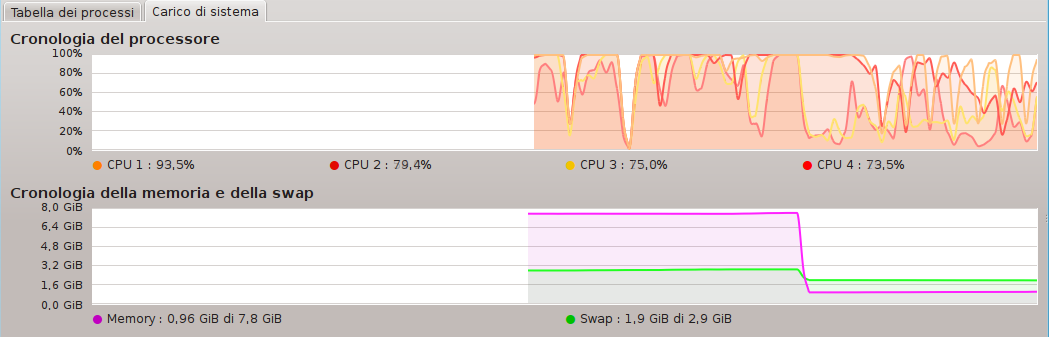
\includegraphics[width=1.0\textwidth]{assets/sib-memory-leak.png}
	\caption{Memory Leak del SIB che avveniva quando la connessione viene interrotta da un socket-timeout}
	\label{fig:sib-memory-leak}
\end{figure}

\noindent
La scoperta di questo problema ha portato quindi alla necessità di ottimizzare le performance, è stato quindi deciso di limitare il numero di risposte fornite dal servizio cittadino (Par. ~\ref{par:thread}) che causa un ingente traffico di dati da e verso il SIB. Altra ottimizzazione che decisa in seguito a queste scoperte è stata quella di trasformare le operazioni di INSERT di triple in query SPARQL, in quanto, grazie all'uso dei prefissi al posto degli URL interi, si riesce ad ottimizzare notevolmente il volume di dati scambiato, il che porta a notevoli vantaggi durante l'uso nell'applicazione mobile.























